%! Author = taj
%! Date = 7/22/25

% Preamble
\documentclass[11pt]{article}

% Packages
\usepackage{amsmath}
\usepackage{graphicx}
\usepackage{float}

\title{3. Idealni plin}
\author{Taj Šobot}

% Document
\begin{document}
    \maketitle
    \flushleft

    V tem eksperimentu smo preverjali veljavnost splošne plinske enačbe.
    V prvem delu smo zrak v posodi segrevali ter merili temperaturo in tlak.
    V drugem pa smo zrak samo počasi enakomerno stiskali, ter merili spremembo tlaka.

    \section{Meritve, rezultati in grafi}

    \subsection{Segrevanje posode}

    Posodo z zrakom smo segrevali.
    Tlak v posodi smo merili z u cevko.
    Prostornina zraka v posodi je bila:

    \[
        V_z = (1000 \pm 1) cm^2
    \]
    Takrat je bil zračni tlak sobe:
    \[
        p_0 = (102 \pm 1)kPa
    \]

    Tlak v posodi smo merili za vsake 2 stopinji spremembe temperature.
    Tlak smo izračunali iz hidrostatičnega tlaka v u cevkah z enačbo:
    \[
        p = p_0 + \rho g h
    \]
    Spodaj so navedene meritve temperature ($T$), spremembe višin u cevkl ($\Delta h$), tlak ($p$), volumen ($V$).
    V petem stolpcu pa se nahajajo vrednosti vstavljene v enačbo:
    \[
        \frac{p V}{T}
    \]
    Če plinska enačba velja mora biti izpolnjen spodnji pogoj:
    \[
        \frac{p_0 V_0}{T_0} = \frac{p_1 V_1}{T_1} = ... = nR = konst
    \]
    \begin{table}[H]
        \centering
        \begin{tabular}{|c|c|c|c|c|}
            \hline
            $T [^\circ]$ & $\Delta h [cm]$ & $\Delta p [Pa]$ & $V [dm^3]$ & $\frac{p V}{T}$\\
            \hline
            24 &  4.9 & 102480 & 1.005 & 0.347 \\
            26 &  9.5 & 102930 & 1.010 & 0.348 \\
            28 & 13.1 & 103280 & 1.013 & 0.348 \\
            30 & 15.7 & 103540 & 1.016 & 0.347 \\
            32 & 18.4 & 103800 & 1.018 & 0.347 \\
            \hline
        \end{tabular}
        \caption{tabela 1}
        \label{tab:1}
    \end{table}
    Pri tem so sledeče napake:
    \begin{align*}
        T_{err} = \pm 1 K \\
        h_{err} = \pm 0.2 cm \\
        p_{err} = \pm 80 Pa \\
        V_{err} = \pm 0.002 dm^3
    \end{align*}

    Kot vidimo iz 5\. stolpca vrednosti odstopajo manj kot 1/3 1\%.
    Potrdili smo veljavnost zgornje enačbe.

    Gremo še preverit za enačbo:
    \[
        A = \frac{dp}{p} + \frac{dV}{V} - \frac{dT}{T} = 0
    \]

    Differencialne spremembe bojo razlike med meritvami.
    Te so v sledeči tabeli (označeni z $\Delta$):

    \begin{table}[H]
        \centering
        \begin{tabular}{|c|c|c|c|}
            \hline
            $\Delta p [pa]$ & $\Delta V [cm^3]$ & $\Delta T [K]$ & A \\
            \hline
            -449 & -4.6 & -2 & -0.00223 \\
            -352 & -3.6 & -2 & -0.00029 \\
            -254 & -2.6 & -2 &  0.00161 \\
            -264 & -2.7 & -2 &  0.00139 \\
            \hline
        \end{tabular}
        \caption{tabela 2}
        \label{tab:2}
    \end{table}

    Vse vrednosti "A" so blizu 0.
    Tudi tukaj vidimo, da se splošna plinska enačba strinja z eksperimentalnimi vrednostmi.

    \subsection{Stiskanje posode}

    V tem delu vaje smo imeli posodo v kateri je bil zrak.
    Prostornine posode smo zmanjševali počasi, da smo dosegli lepo izotermno spremembo.
    \\
    Polmer bata je bil izmerjen $r_{bata} = (2,0 \pm 0,1) cm$.
    Njegova površina je torej bila:
    \[
        A = \pi r_{bata}^2 =(12.6 \pm 0.6)cm^2
    \]
    Naredili smo 10 meritev po korakih 0,10 bar in merili za koliko smo stisnili plin v posodi.
    Meritve v spodnji preglednici (in izračunan volumen):
    \begin{table}[H]
        \centering
        \begin{tabular}{|c|c|c|}
            \hline
            $p [bar]$ & $l [cm]$ & $V [cm^3]$\\
            \hline
            1.05 & 25.0 & 3.2  \\
            1.1 & 24.0  & 3.0  \\
            1.2 & 21.7  & 2.7  \\
            1.3 & 19.7  & 2.5  \\
            1.4 & 18.2  & 2.3  \\
            1.5 & 16.8  & 2.1  \\
            1.6 & 15.8  & 2.0  \\
            1.7 & 14.9  & 1.9  \\
            1.8 & 14.0  & 1.8  \\
            1.9 & 13.2  & 1.7  \\
            2.0 & 12.6  & 1.6  \\
            \hline
        \end{tabular}
        \caption{tabela 3}
        \label{tab:3}
    \end{table}


    Napake meritev:
    \begin{align*}
        p_{err} = \pm 0.1 bar \\
        l_{err} = 0.1 cm \\
        V_{err} = 0.1 cm^2
    \end{align*}

    Spodaj je še graf meritev p(V):
    \begin{figure}[H]
        \centering
        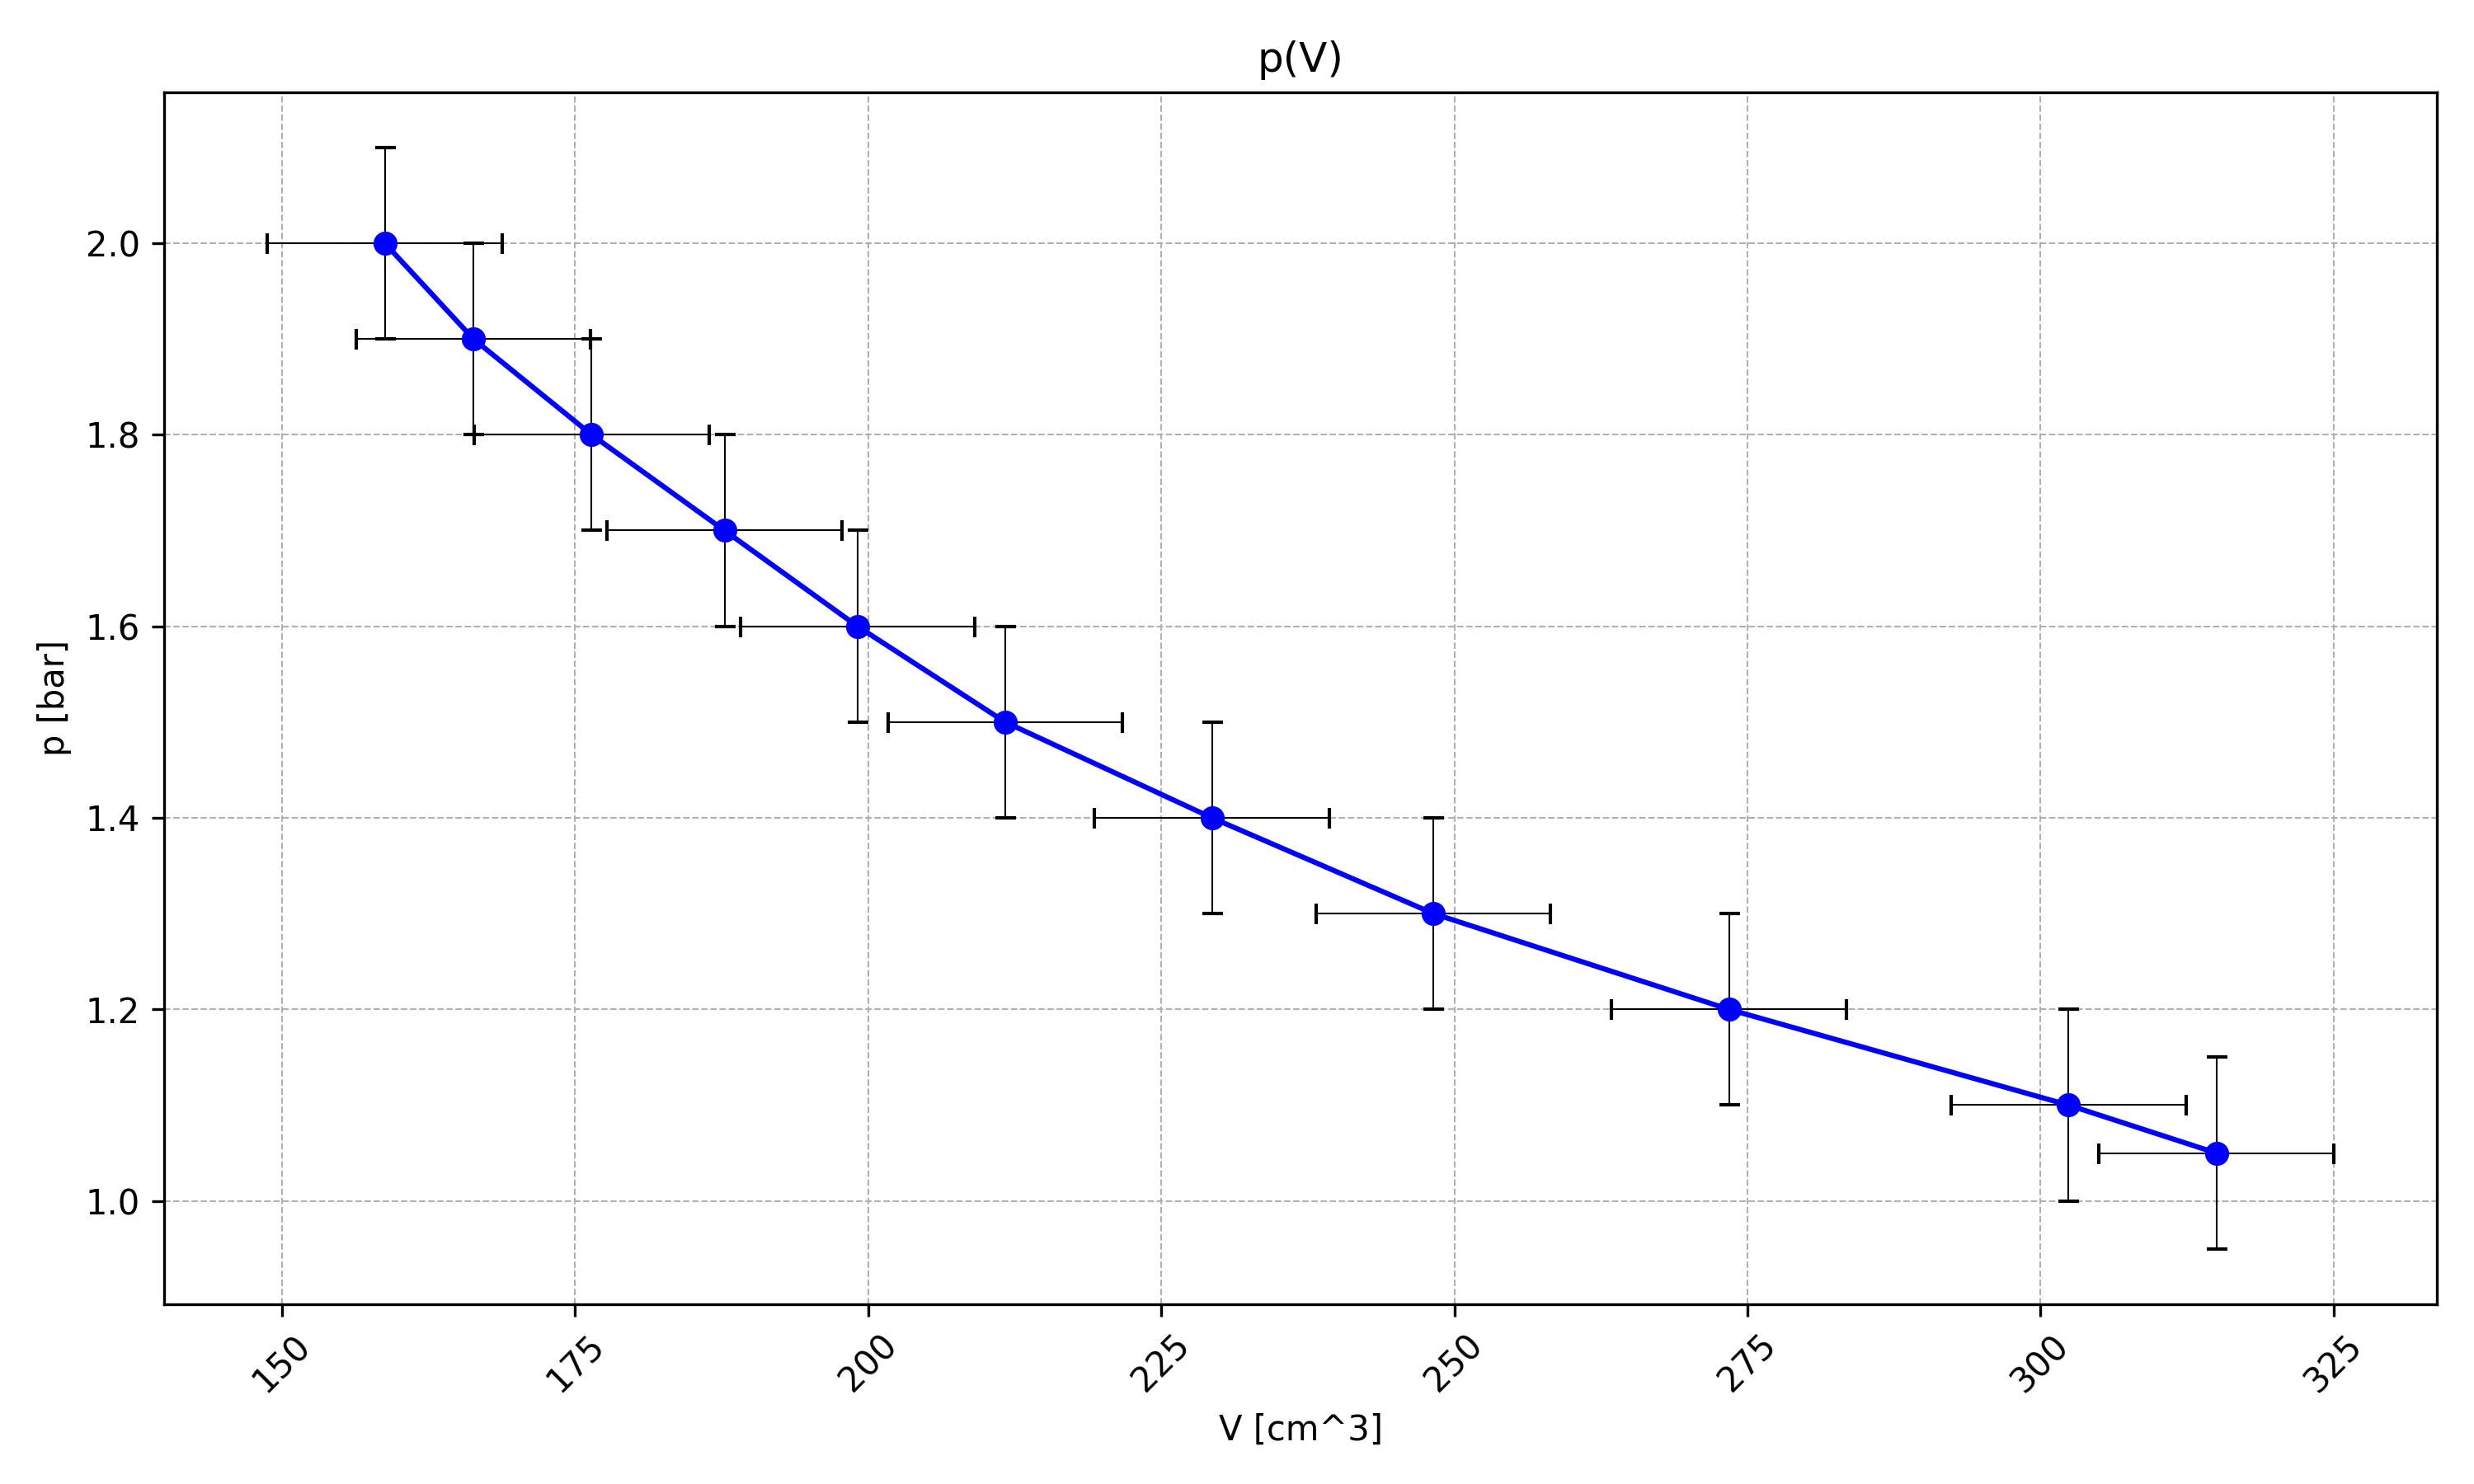
\includegraphics[width=0.9\textwidth]{2del2}
        \caption{Graf 1}
        \label{fig:1}
    \end{figure}

    In še lineariziran graf p(1/V).
    \begin{figure}[H]
        \centering
        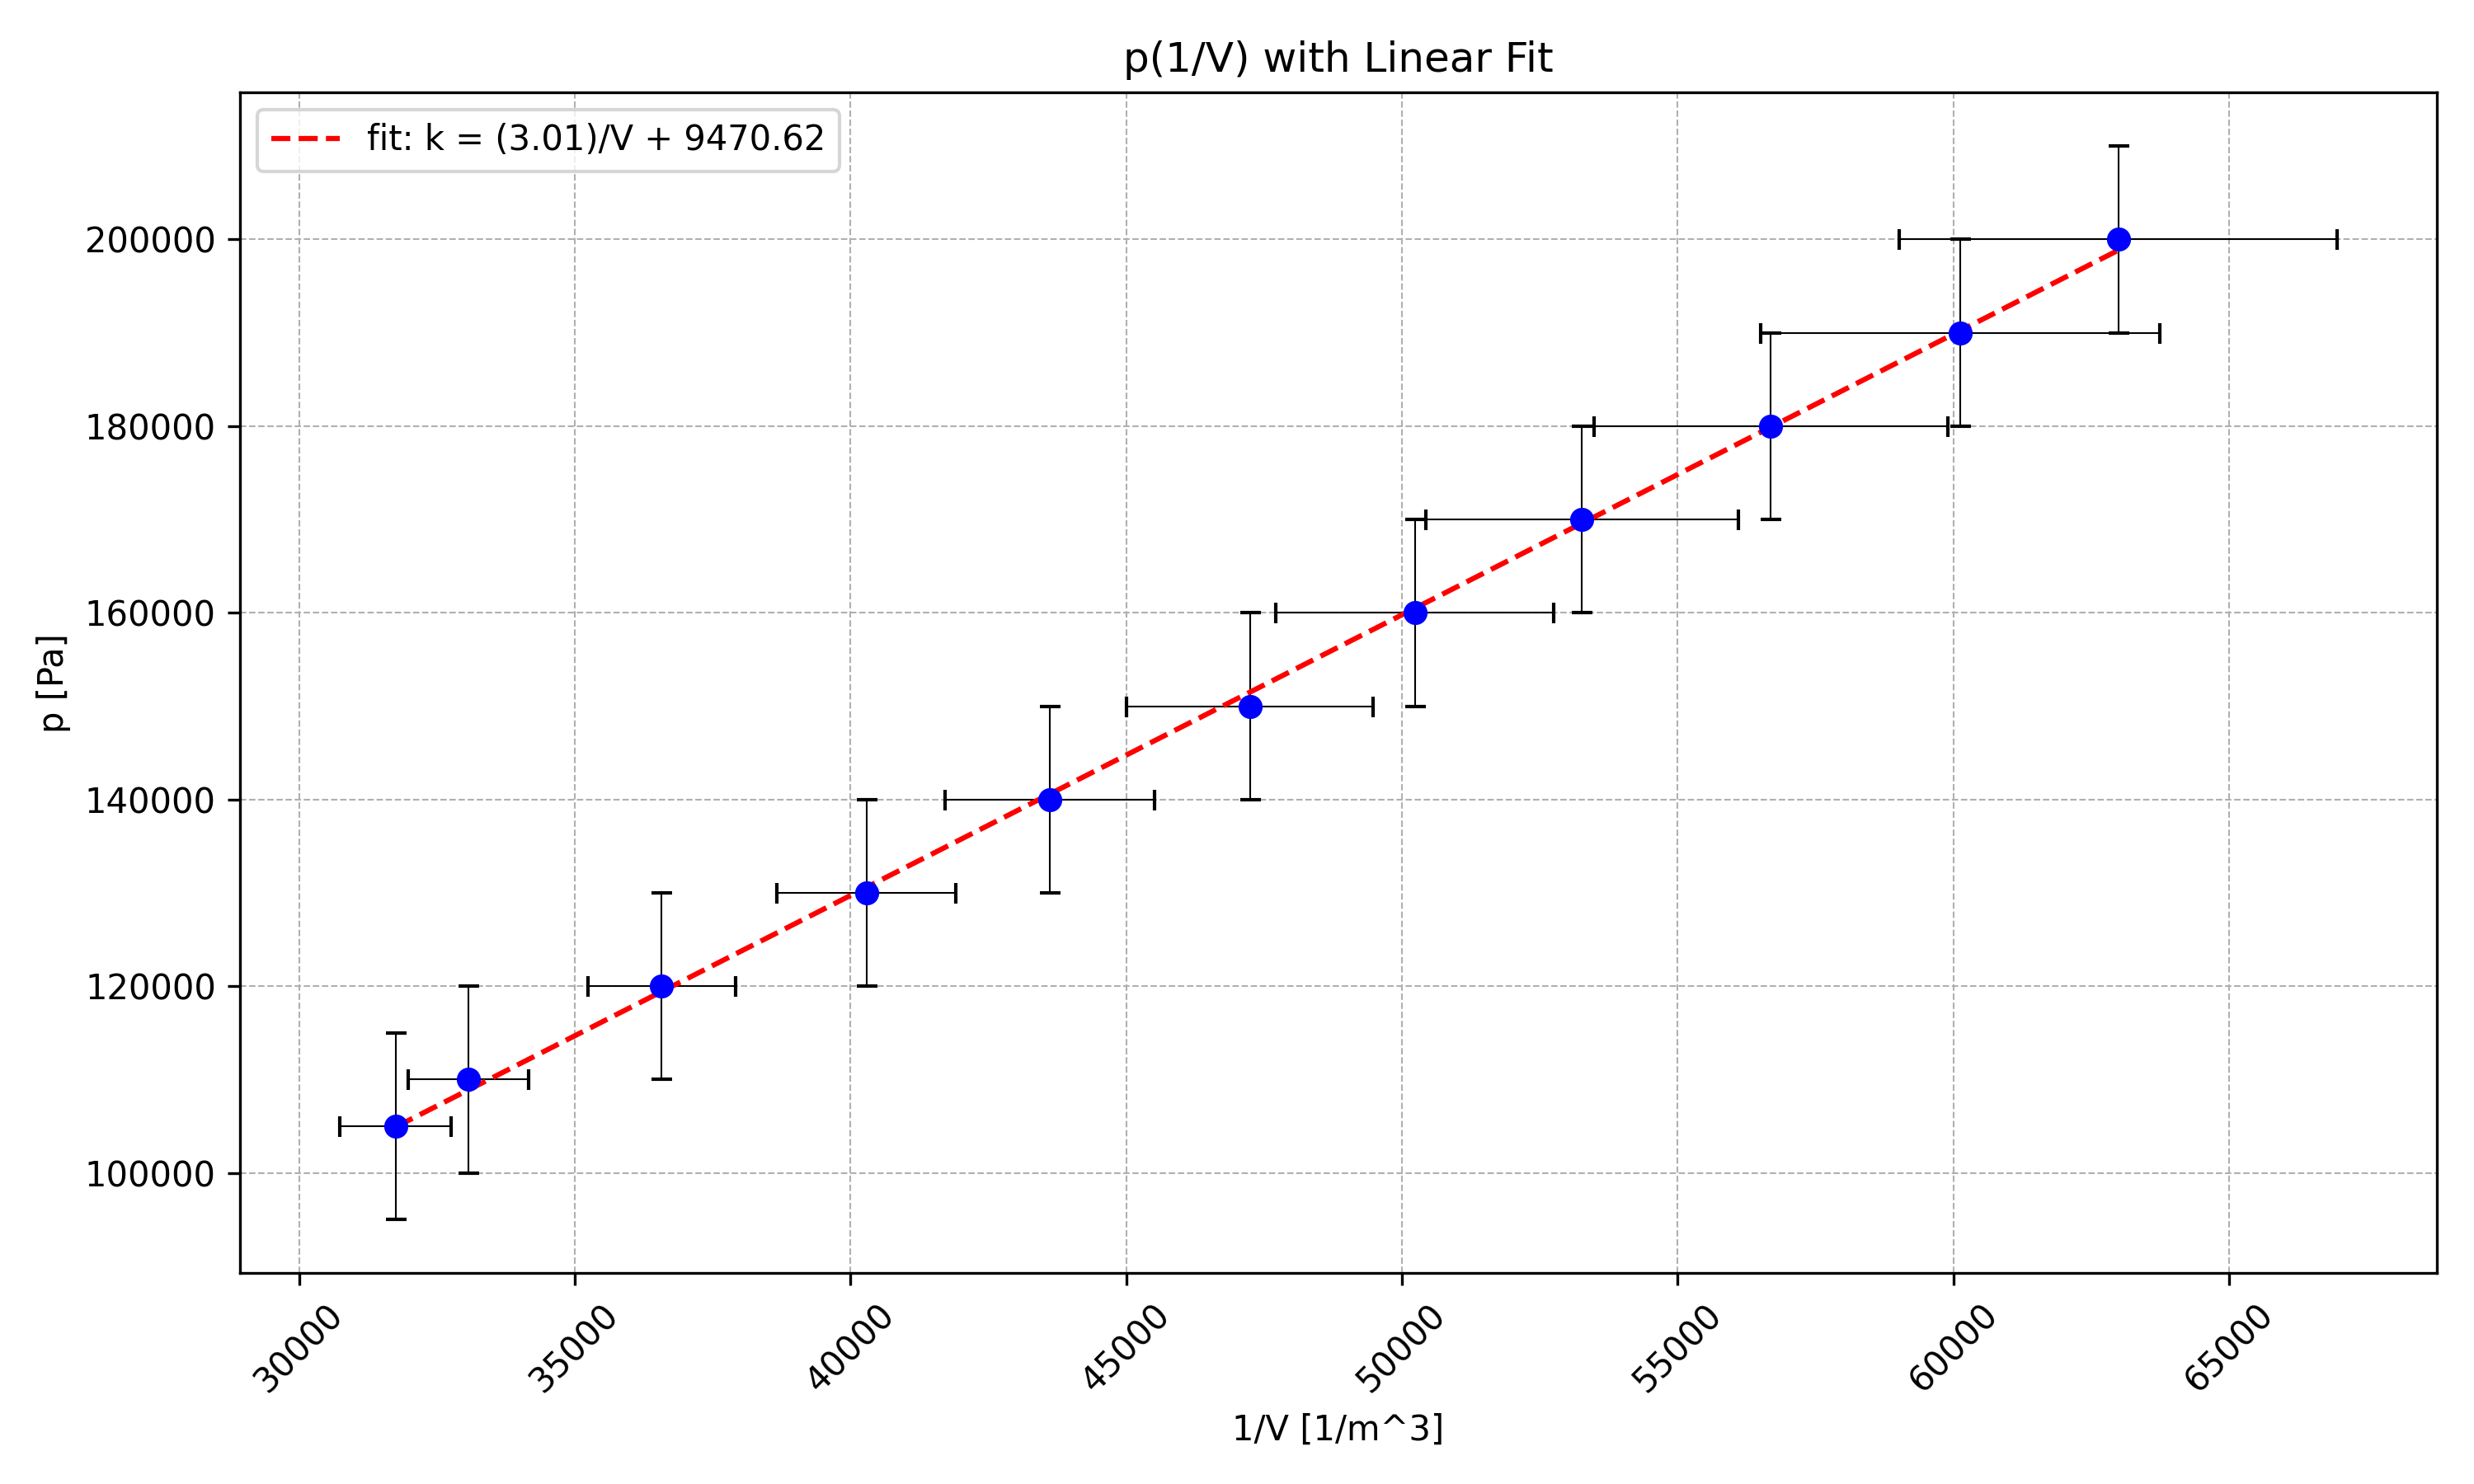
\includegraphics[width=0.9\textwidth]{2del3_with_fit}
        \caption{Graf 2}
        \label{fig:2}
    \end{figure}
    Iz tega lahko odčitamo koeficient.
    Ta je enak produktu $k = nRT$.
    Torej če hočemo izračunati R sledi:
    (vstavimo $k = (3.01 \pm 0.8) Pa m^3 $, $T = (294 \pm 1) K$ in $n = 0.014$)
    \[
        R = k/(nT) = (7.9 \pm 0.2)  \frac{J}{K mol}
    \]

    Komentar:
    Realna vrednost splošne plinske konstante je 8.314, lahko opazimo malo odstopanje, ki ni znotraj napake.
    Nekatere meritve so mogoče mele večje napake kot pričakovane.

    \section{Odgovori na vprašanja}
    \textit{Za katere pline bi lahko z dano napravo preveril veljavnost plinske enačbe? (navezuje na 1. del)}
    \\
    Za vse pline, ki so plini pri sobni temperaturi ($\pm 20 K$), da nam voda v u cevkah in aparatu ne zmrzne ali se izpari...
    Tudi pline, ki niso zelo redki pri sobnih pogojih, recimo helij ali vodik.
    \textit{Kako je tlak odvisen od prostornine pri adiabatni spremembi? Zapišite zvezo in
    skicirajte odvisnost!}
    \\
    Odvisnost: $pV^\gamma = konst.$
    graf odvisnosti:
    \begin{figure}[H]
        \centering
        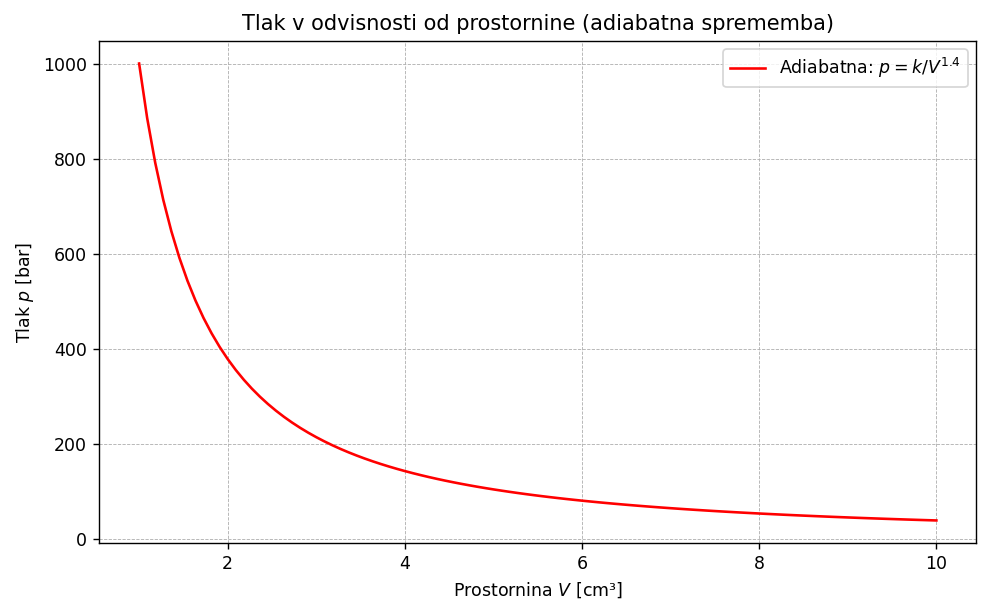
\includegraphics[width=0.9\textwidth]{adiabata}
        \caption{Graf 3}
        \label{fig:3}
    \end{figure}
\end{document}